\documentclass[11pt]{article} 
\usepackage{geometry}
\geometry{letterpaper}

\usepackage{graphicx}   
\usepackage{amssymb}
\usepackage{float}
\usepackage{tabularx}
\usepackage{multicol}
\usepackage{hyperref}
\hypersetup{
    colorlinks,
    citecolor=black,
    filecolor=black,
    linkcolor=black,
    urlcolor=black
}

\begin{document}

\begin{titlepage}
	\newcommand{\HRule}{\rule{\linewidth}{0.2mm}}
	\begin{center}
	\textsc{\LARGE McMaster University}\\[1.5cm]
	
	\textsc{\Large SmartServe}\\[0.5cm]
	\textsc{\large Software \& Mechatronics Capstone}\\[0.5cm] 

	\HRule\\[0.4cm]
		{\huge\bfseries High Level System Design}\\[0.4cm]
	\HRule\\[0.4cm]
	
	\begin{minipage}[t][][t]{0.5\textwidth}
		\begin{flushleft} \large
			\emph{Authors:}\\
			Christopher McDonald\\
			Harit Patel \\
			Janak Patel \\
			Jared Rayner  \\
			Nisarg Patel  \\
			Sam Hamel \\
			Sharon Platkin \\
		\end{flushleft}
	\end{minipage}
	~
	\begin{minipage}[t][][t]{0.4\textwidth}
		\begin{flushright} \large
			\emph{Professor:} \\
			Dr. Alan Wassyng \\[0.4cm]
			\emph{Teaching Assistants:} \\
			Bennett Mackenzie \\ 
			Nicholas Annable \\ 
			Stephen Wynn-Williams \\ 
			Viktor Smirnov
		\end{flushright}
	\end{minipage}\\[2cm]
	
	
\includegraphics[width=0.3\textwidth]{logo.png} \\
	{\large Last compiled on \today}
	\end{center}

\end{titlepage}

\tableofcontents
\listoffigures

\vfill
\begin{figure}[H]
   \centering
   \noindent\begin{tabularx}{\textwidth}{| >{\centering\arraybackslash}m{0.2\textwidth} | >{\centering\arraybackslash}m{0.2\textwidth} | >{\centering\arraybackslash}m{0.2\textwidth} | >{\centering\arraybackslash}m{0.285\textwidth} |}
   \hline 
   \textbf{Date} & \textbf{Revision} & \textbf{Comments} & \textbf{Author(s)} \\ \hline
   Dec 1, 2017 & 1.0 & Main content done for all sections & Christopher McDonald \\ \hline
   Dec 13, 2017 & 1.1 & Corrected Document Overview & Nisarg Patel \\ \hline
   Dec 14, 2017 & 1.2 & Refined Project Scope & Nisarg Patel \\ \hline
   \end{tabularx}
   \caption{Revision History}
\end{figure}
\newpage
\section{Introduction}
% todo pass mode to shot recommendation system
\subsection{Project Overview}
SmartServe is an autonomous table tennis training system for table tennis players with various skill levels. SmartServe aids in diagnosing and improving a player's performance over time. The system trains table tennis players by shooting table tennis balls towards the player and detects successful returns from the player. The system can further adapt to the player's weaknesses and help them overcome it through further training. Importantly, SmartServe alleviates the problems of finding and working with a coach for players, as well as coaches trying to train multiple players simultaneously. The system will be deemed a success if the table tennis players and coaches, can enjoy and see a value added by using SmartServe.\\\\
The project started at the beginning of the Fall 2017 academic term and will conclude at the end of the Winter 2018 term. In addition, the core project team consists of final year Software and Mechatronics Engineering students who are enrolled in the MECHTRON 4TB6/SFWRENG 4G06 capstone project course.
\subsection{Document Overview}
The purpose of this document is to provide an overview of the team's proposed system design that meets the system requirements as specified in the Requirements document (SRS). After reading this document, the reader should have a clear understanding of system/subsystem interactions, different subsystems, roles and uses of subsystems, as well as how the proposed system design will address the requirements. \\ \\
At first, the system is decomposed into subsystems while highlighting each subsystems own responsibilities and design. Next, the document outlines the subsystems intended inputs, expected outputs and description of its use. Later, the document details the expected use cases to understand user expectations and subsystem interactions in the Sequence Diagram section. For every subsystem, this document defines its purpose with respect to the overall system. Later, detailed input and output parameters are defined. The means of communication are also described as these could be simple method calls to requests over some transport protocol like HTTP or TCP. The architecture for each subsystem will be designed in the low level design document. These decisions will be based on the unique requirements each subsystem needs to satisfy. At the end of this document, each subsystem is responsible for implementing some set of requirements. Those requirements are outlined in the requirements document found here. % TODO link
Please note that in the ideal scenario, one subsystem will be the only one that is responsible for any one requirement but may not be the case for all of the requirements. 

\subsection{Naming Conventions and Terminology}
\label{sec:definitions}
The following terms and definitions will be used throughout this document:
\begin{itemize}
% Alphabetical order is highly preferred as it eases user navigation
\item \textbf{ACID}: a database transaction which is atomic, consistent, isolated and durable
\item \textbf{CV}: computer vision subsystem to perform image processing
\item \textbf{FPS}: frames per second
\item \textbf{GUI}: graphical user interface
\item \textbf{HTTP:} hypertext transfer protocol
\item \textbf{Pitch}: rotation along the y-axis; this rotation angle primarily dictates the range of the ball from the net to the edge of the table on the user side
\item \textbf{Roll}: rotation along the x-axis
\item \textbf{Shooting Mechanism}: refers to the part of the system that shoots the table tennis balls towards the user side (player). Please refer to Figure \ref{fig:table-tennis-top-view} for visual illustration.
\item \textbf{System Side}: the side of the table where the electromechanical system is placed; it is the opposite side of the User Side. Please refer to Figure \ref{fig:table-tennis-top-view} for visual illustration.
\item \textbf{System}: encompasses both the hardware and software parts of SmartServe
\item \textbf{TCP:} transmission control protocol
\item \textbf{Team}: all team members of the core capstone project, as noted in the list of Authors
\item \textbf{User Side}: the side of the table where the user (player) is standing
\item \textbf{Yaw}: rotation along the z-axis; this rotation angle primarily dictates the panning functionality of the shooting mechanism from the right side to the left side of the table
\end{itemize}

\begin{figure}[H]
   \centering
   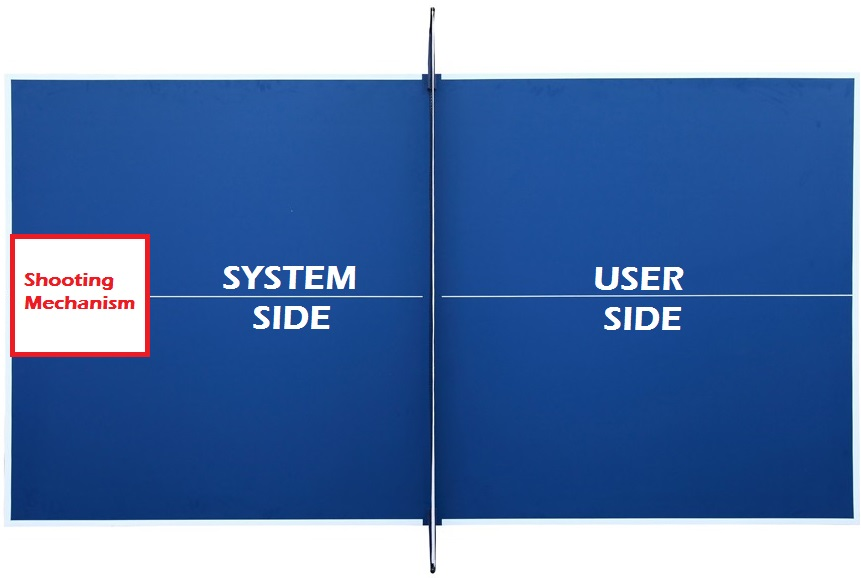
\includegraphics[width=0.75\textwidth]{img/Table-Tennis-Top-View.png} %requires the graphicx package
   \caption{Top View of the Tennis Table}
   \label{fig:table-tennis-top-view}
\end{figure}
\subsection{Project Scope}
The system will only attempt to shoot balls from the shooting mechanism straight towards the user side. Importantly, the system will not attempt to return any shots from the user. After the user has returned a shot, the Computer Vision (CV) subsystem will be utilized to determine if the user's shot lands on the table or not. Additionally, the characteristics of the shot following any return will be determined by the system's mode and the proficiency of the player if available.
\section{System Description}
\subsection{System Architecture}
The system will follow a service-oriented / process-based architecture. This means that a central subsystem will interface with several services that serve a single purpose. Some subsystems will be simply told what needs to be done and others will asked for some return value. This is done to implement separation of concerns where one subsystem doesn't know everything about the system and only what is necessary to satisfy their requirements. It also allows for easy increments of versioning, where one subsystem can be used as long as it is functional and easily swapped out for a newer version with extra features or increased performance. Moreover, this system has heavy timing constraints and an unpredictable environment so some actions must be taken in absence of a service's response. For example, the computer vision may take longer to track a ball depending on its trajectory where the system must shoot another ball in order to keep the user engaged.

\subsection{Subsystems Overview}
The system will be broken down into the subsystems with the following purposes: general managing of subsystems, computer vision to detect returns, shot recommendation, model the shot's trajectory, optimize the distance travelled by the shooting mechanism, store the data, take input and output from the user and shooting the ball toward the user. The diagram for this breakdown can be found in Figure \ref{fig:sub}.
\begin{figure}[H]
   \centering
   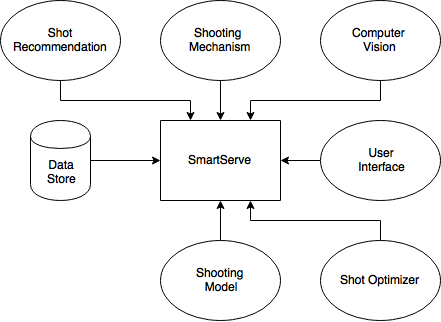
\includegraphics[width=0.6\textwidth]{img/Subsystem.png} % requires the graphicx package
   \caption{Subsystem Breakdown}
   \label{fig:sub}
\end{figure}
\subsubsection{Smart Serve}
The Smart Serve subsystem will provide the means of interfacing with all the subsystems and enforcing timing constraints. For all intents and purposes, it can be considered the main process and hub of the system. In the event a subsystem is taking too long to respond, this subsystem must be able to continue operation to meet timing requirements. The various states and transitions can be found in Figure \ref{fig:fsm}. The FSM diagram shows each state should have an \textit{exit option} if a service takes longer than allowed to preform an action.
\begin{figure}[htbp]
   \centering
   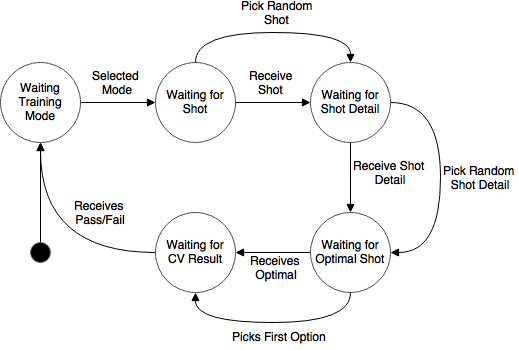
\includegraphics[width=0.7\textwidth]{img/FSM.png}
   \caption{Smart Serve FSM}
   \label{fig:fsm}
\end{figure}

\subsubsection{Computer Vision}
The Computer Visions subsystem will be a service to the Smart Serve subsystem to determine if a shot is successfully returned. When sent a request to begin tracking the ball, it will do so and return a true or false when the ball bounces off the table or it doesn't. In the event the ball never enters frame, it will assume the return was failed after a fixed amount of time.

\subsubsection{Shot Recommendation}
The Shot Recommendation subsystem will be a service to the Smart Serve subsystem to determine which shot should be taken next. The way the subsystem decides on the shot will be determined by the training mode the user selects. These will include shooting the same shot every time, pseudo-randomly picking a shot or using reinforcement learning algorithms to decide the next shot. The last mode will be based on previous performance by the user.

\subsubsection{Shooting Model}
The Shooting Model subsystem will be a service to the Smart Serve subsystem which provides the means of mapping a desired shot to the details needed to take the shot. The input and output for the system can be found in Figure \ref{fig:shotmodel}. The output will be many combinations of pitch, yaw, speed and angular velocity that satisfy the input shot details. 
\begin{figure}[htbp]
   \centering
   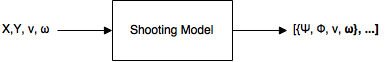
\includegraphics[width=0.6\textwidth]{img/ShotModel.png} % requires the graphicx package
   \caption{Shooting Model I/O}
   \label{fig:shotmodel}
\end{figure}
\subsubsection{Shot Optimizer}
The Shot Optimizer will be a service to the Smart Serve subsystem which provides means of reducing the travel time the shooting mechanism needs to do in order to shoot the desired shot. This will simply scan each possible orientation and pick one which minimizes the distance travelled for the mechanism.
\subsubsection{Data Storage}
The Data Storage subsystem will store all the details for each shot, the user's profile and the return rates for each user. It will need to have interfaces for saving data and querying data out of the system in a variety of formats. Ideally, it will require minimal detail and configuration for the subsystem which uses it due a variety of implementations of these subsystems. 
\subsubsection{User Interface}
The User Interface subsystem will be the means of translating user requests into actionable requests for the Smart Serve subsystem.
\subsubsection{Shooting Mechanism}
The Shooting Mechanism will be the subsystem which actually fires the ball towards the user. A microcontroller will be used as the point of contact and set any actuators required to fire a specified shot. It must complete this action within 1.5 seconds for the Computer Vision to detect the ball returned by the user. 


\subsection{Use Cases}
The diagram including all use cases can be found in Figure \ref{fig:usecase}. The user-instantiated ones will be described in detail below.
\begin{figure}[htbp]
   \centering
   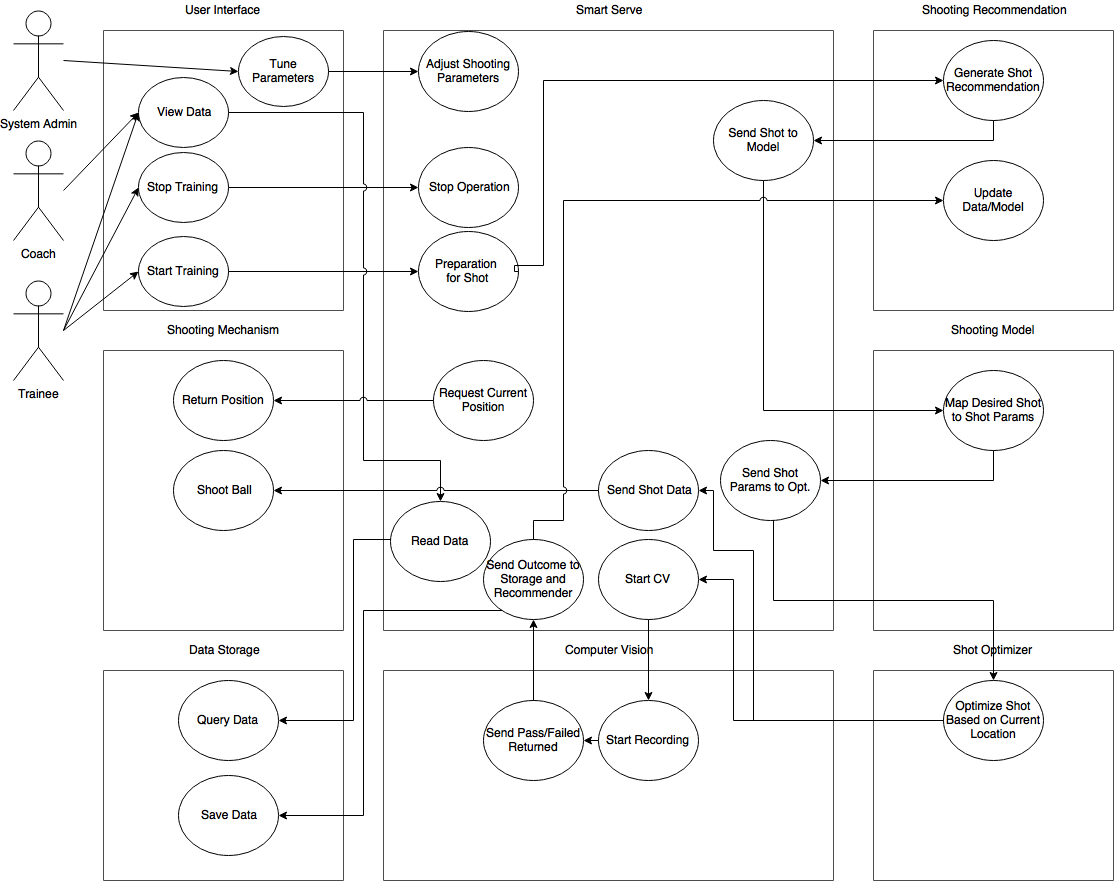
\includegraphics[width=\textwidth]{img/UseCase.png} % requires the graphicx package
   \caption{Use Case Diagram}
   \label{fig:usecase}
\end{figure}
\subsubsection*{Start Training}
The user interface will have ways to allow the user to start this action which makes the Smart Serve subsystem prepare for a shot to fire towards the user. To do this, it needs to request a shot to use from the Shot Recommendation subsystem. This will be in the form of a desired location on the table, the speed of the shot and the angular velocity of the ball. The Smart Serve subsystem can then use the Shooting Model to translate this information into pitch, yaw and angular velocity to shoot the ball so it matches the desired shot. The Smart Serve subsystem can then use the Shooting Mechanism's current position and the desired shot to request the optimal position to shoot the ball using the Shot Optimizer. After doing so, it will instruct the shooting mechanism to shoot the ball in the desired way and start the CV subsystem to begin tracking for a successful return. Only until the CV subsystem returns the pass or failed return data, can it update the Data Storage and Shot Recommendation subsystems with this new information. The former will store the result and the data for the shot together, where the latter will update the model used to generate shot recommendations. After doing all this, it can begin preparing for a new shot.
\subsubsection*{Stop Training}
In the event the user wants to cease training, the user interface will allow this and will halt the system from shooting balls. No data should be written or shots requested for the shooting mechanism to fire in order to preserve the integrity of the data the system gathers.
\subsubsection*{View Results}
When the user wants to visualize the results of their performance, the user interface will allow this action to begin. It will use the Smart Serve subsystem to query data from data storage and present it in some meaningful way.
\subsubsection*{Tune Parameters}
The system made need to be adjusted for various lighting, table sizes or environments. The user interface will allow a system administrator to do this in order to directly change values associated for these variables.
\subsubsection*{Start System}
The user interface will allow the system to be booted where it starts the Smart Serve subsystem. This will read allow the Shot Recommendation system to build its model based on previous data for the user, if it exists.
\subsection{Sequence Diagram}
The sequence diagram for each user-initiated use case are listed below in their respective sections.
\subsubsection*{Start Training}
\begin{figure}[htbp]
   \centering
   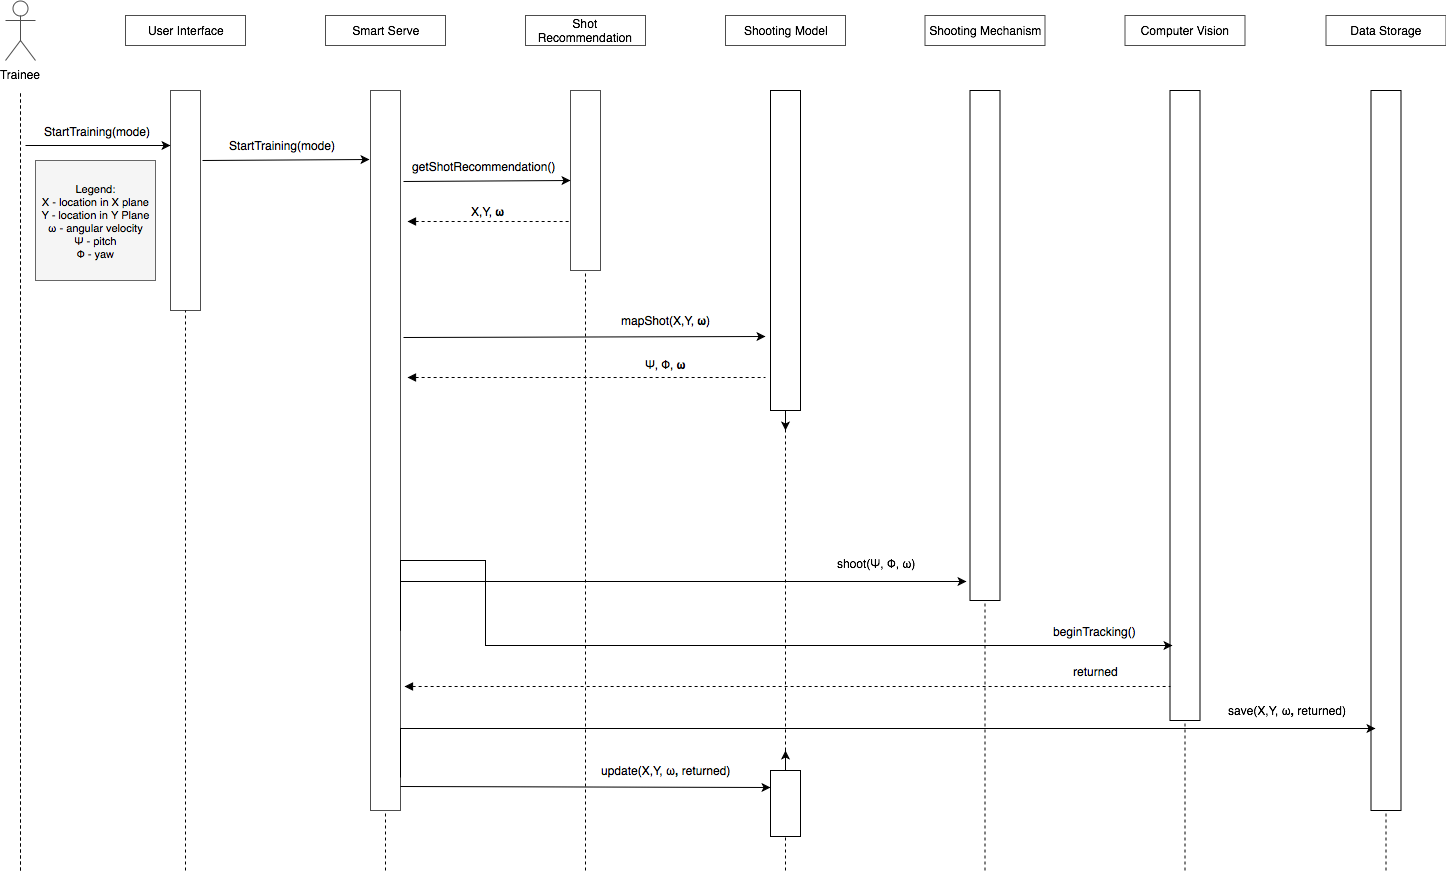
\includegraphics[width=\textwidth]{img/SequenceDiagram-Start.png}
   \caption{Sequence Diagram for Starting Training}
   \label{fig:start}
\end{figure}
\subsubsection*{Stop Training}
\begin{figure}[htbp]
   \centering
   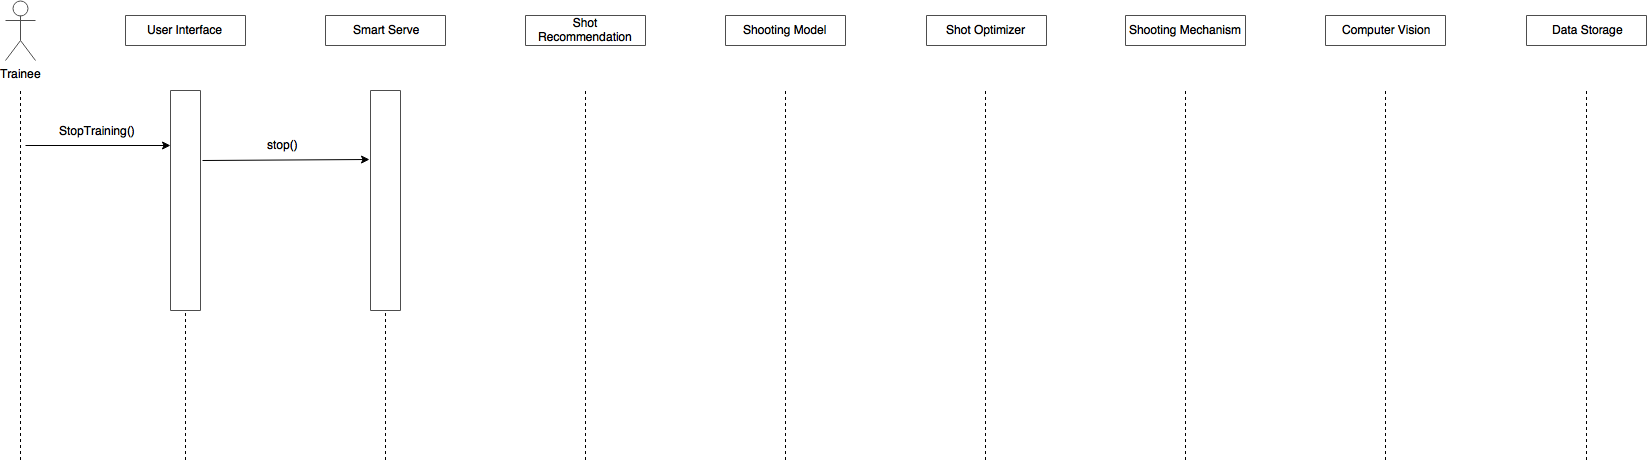
\includegraphics[width=\textwidth]{img/SequenceDiagram-Stop.png}
   \caption{Sequence Diagram for Ceasing Training}
   \label{fig:stop}
\end{figure}
\subsubsection*{View Results}
\begin{figure}[htbp]
   \centering
   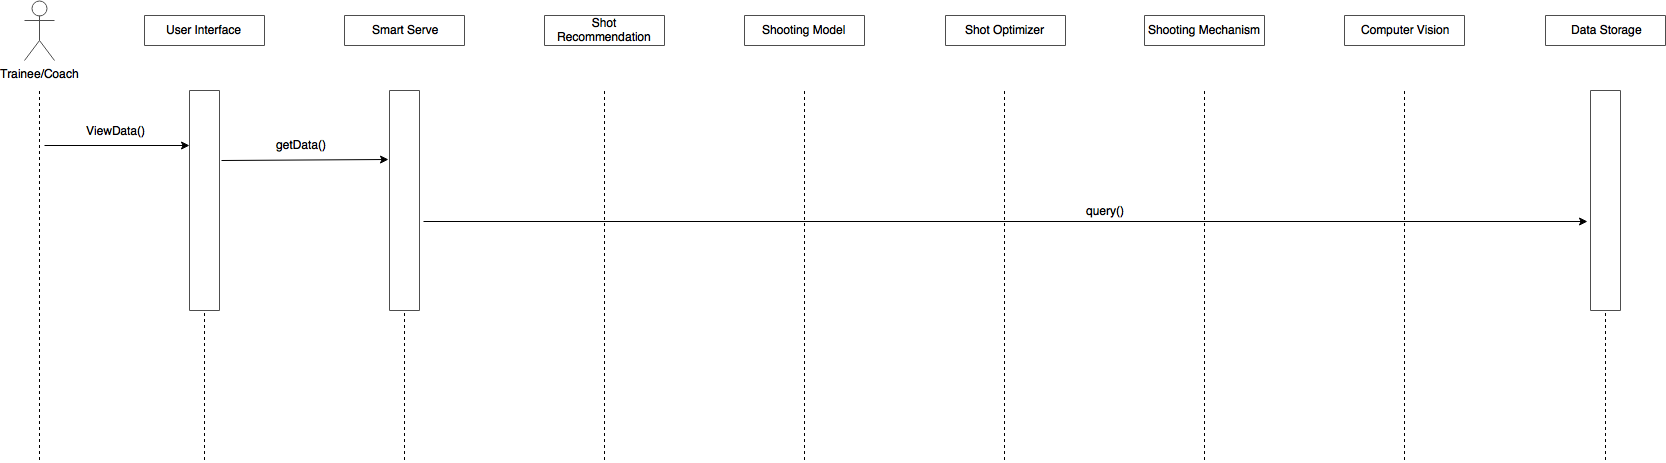
\includegraphics[width=\textwidth]{img/SequenceDiagram-View.png}
   \caption{Sequence Diagram for Viewing Training Results}
   \label{fig:view}
\end{figure}
\subsubsection*{Tune Parameters}
\begin{figure}[htbp]
   \centering
   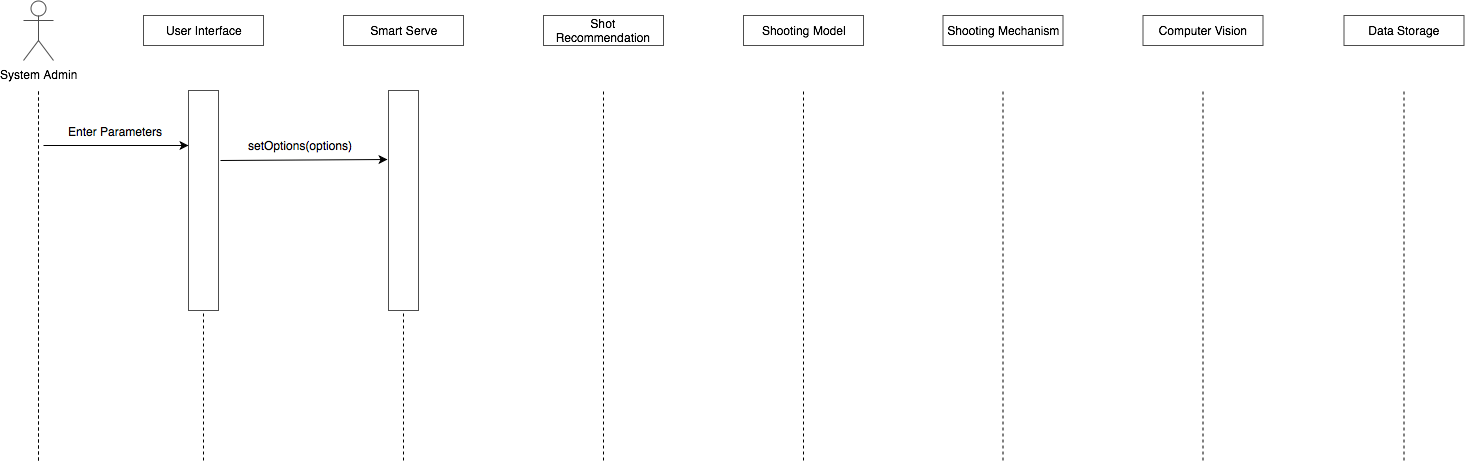
\includegraphics[width=\textwidth]{img/SequenceDiagram-Tune.png}
   \caption{Sequence Diagram for Tuning Parameters}
   \label{fig:tune}
\end{figure}
\subsubsection*{Start System}
\begin{figure}[H]
   \centering
   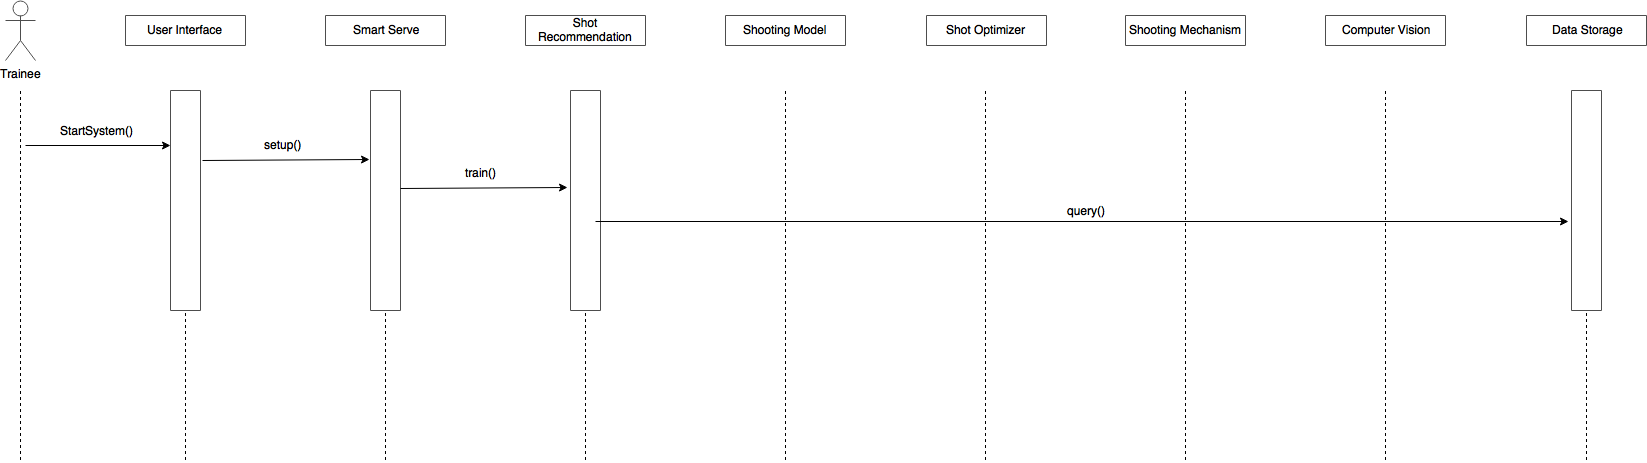
\includegraphics[width=\textwidth]{img/SequenceDiagram-Boot.png}
   \caption{Sequence Diagram for Booting the System}
   \label{fig:boot}
\end{figure}
\subsection{Behaviour Description}
As the behaviour of the system has been discussed previously, this section will describe the expected user behaviour and how they would interact with the system.
\subsubsection{Normal Operation}
The trainee would begin by starting the system from its off state. This will trigger the Start System use case and allow the Smart Serve system to boot and the Shot Recommendation System to boot and build a model to recommend shots. The user will then trigger the Start Training use case and specify a training mode. This creates the loop of Smart Serve prepping and serving shots for the user. Only until the user starts the Stop System use case will this loop stop during normal operation. Either during training or after, a user can start the View Data use case to get details on their performance.
\subsubsection{Error Handling}
If the system should encounter an error, it should display the details of it through the User Interface subsystem. In addition to this, it must take measures to ensure the safety of the user and integrity of the system. This includes stopping all training and pending actions for the system to perform. For example, an error could be a jammed table tennis ball or the system has run out of balls to use.
\section{Class Responsibility Collaboration (CRC) Cards}
\subsection{SmartServe}
\begin{table}[H]
\centering
\label{my-label}
\begin{tabular}{ | p{0.4\textwidth} | p{0.4\textwidth} | }
\hline
\multicolumn{2}{|c|}{\textbf{Smart Serve}}             \\ \hline
\textbf{Responsibilities:} & \textbf{Collaborators:} \\ \hline
\begin{itemize} 
\item \textbf{F10}: pause the shooting mechanism
\item \textbf{F18}: shoot a ball once the previous has been returned to the system side or 1.5 seconds after the previous shot, whichever is shorter
\item \textbf{P2}:  must include all but previous 3 shots in performance data
\item \textbf{P5}: must support only one user playing at one time
\end{itemize} 
& 
\begin{itemize} 
\item Computer Vision
\item Shot Recommendation
\item Shooting Model
\item Shot Optimizer
\item Data Storage
\item User Interface
\item Shooting Mechanism
\end{itemize} \\ \hline
\end{tabular}
\caption{Smart Serve CRC Card}
\end{table}

\subsection{Computer Vision}

\begin{table}[H]
\centering
\label{my-label}
\begin{tabular}{ | p{0.4\textwidth} | p{0.4\textwidth} | }
\hline
\multicolumn{2}{|c|}{\textbf{Smart Serve}}             \\ \hline
\textbf{Responsibilities:} & \textbf{Collaborators:} \\ \hline
\begin{itemize}
\item \textbf{F5}: detect a successful return by the user
\item \textbf{OE2}: functional in indoor settings with bright florescent lighting
\end{itemize} 
& 
\begin{itemize} \item Smart Serve
\end{itemize} \\ \hline
\end{tabular}
\caption{Computer Vision CRC Card}
\end{table}

\subsection{Shot Recommendation}

\begin{table}[H]
\centering
\label{my-label}
\begin{tabular}{ | p{0.4\textwidth} | p{0.4\textwidth} | }
\hline
\multicolumn{2}{|c|}{\textbf{Smart Serve}}             \\ \hline
\textbf{Responsibilities:} & \textbf{Collaborators:} \\ \hline
\begin{itemize} 
\item \textbf{F7}: load a previously saved state
\item \textbf{MS1}: must support adding different modes to the system
\end{itemize} 
& 
\begin{itemize} 
\item Smart Serve
\item Data Storage
\end{itemize} \\ \hline
\end{tabular}
\caption{Shot Recommendation CRC Card}
\end{table}

\subsection{Shooting Model}

\begin{table}[H]
\centering
\label{my-label}
\begin{tabular}{ | p{0.4\textwidth} | p{0.4\textwidth} | }
\hline
\multicolumn{2}{|c|}{\textbf{Smart Serve}}             \\ \hline
\textbf{Responsibilities:} & \textbf{Collaborators:} \\ \hline
\begin{itemize} 
\item \textbf{F13}: implements a training mode
\item \textbf{F14}: implements a one-shot mode
\end{itemize} 
& 
\begin{itemize} 
\item Smart Serve
\end{itemize} \\ \hline
\end{tabular}
\caption{Shooting Model CRC Card}
\end{table}

\subsection{Shot Optimizer}

\begin{table}[H]
\centering
\label{my-label}
\begin{tabular}{ | p{0.4\textwidth} | p{0.4\textwidth} | }
\hline
\multicolumn{2}{|c|}{\textbf{Smart Serve}}             \\ \hline
\textbf{Responsibilities:} & \textbf{Collaborators:} \\ \hline
N/A & \begin{itemize} \item Smart Serve \end{itemize} \\ \hline
\end{tabular}
\caption{Shot Optimizer Card}
\end{table}

\subsection{Data Storage}

\begin{table}[H]
\centering
\label{my-label}
\begin{tabular}{ | p{0.4\textwidth} | p{0.4\textwidth} | }
\hline
\multicolumn{2}{|c|}{\textbf{Smart Serve}}             \\ \hline
\textbf{Responsibilities:} & \textbf{Collaborators:} \\ \hline
\begin{itemize} 
\item \textbf{F6}: saves details for each shot taken by the shooting mechanism 
\item \textbf{F8}: allows creation of a new user
\item \textbf{F9}: authenticate users
\item \textbf{P4}: must support 1000 users
\item \textbf{MS2}: able to add new metrics to analyze performance
\item \textbf{S1}: hash all passwords for user profiles
\item \textbf{S2}: encrypt all performance data for each user
\item \textbf{P1}: allow read access for coaches
\end{itemize} 
& 
\begin{itemize} 
\item Shot Recommendation
\item Smart Serve
\end{itemize} \\ \hline
\end{tabular}
\caption{Data Storage CRC Card}
\end{table}

\subsection{User Interface}

\begin{table}[H]
\centering
\label{my-label}
\begin{tabular}{ | p{0.4\textwidth} | p{0.4\textwidth} | }
\hline
\multicolumn{2}{|c|}{\textbf{Smart Serve}}             \\ \hline
\textbf{Responsibilities:} & \textbf{Collaborators:} \\ \hline
\begin{itemize} 
\item \textbf{F11}: end the training session
\item \textbf{F12}: resume training session from a paused state
\item \textbf{F13}: display user's performance over a custom time range
\item \textbf{F16}: allows user to adjust training parameters during an active or paused session
\item \textbf{F17}: can be calibrated for a specific table size
\item \textbf{LF1}: have a minimalist design that is easy to navigate through
\item \textbf{UH1}: is intuitive to use
\item \textbf{UH2}: operable using the English language
\item \textbf{P1}: response time for user input must be less than or equal to 100ms
\end{itemize} 
& 
\begin{itemize} 
\item Smart Serve
\end{itemize} \\ \hline
\end{tabular}
\caption{User Interface CRC Card}
\end{table}

\subsection{Shooting Mechanism}

\begin{table}[H]
\centering
\label{my-label}
\begin{tabular}{ | p{0.5\textwidth} | p{0.5\textwidth} | }
\hline
\multicolumn{2}{|c|}{\textbf{Smart Serve}}             \\ \hline
\textbf{Responsibilities:} & \textbf{Collaborators:} \\ \hline
\begin{itemize}
\item \textbf{F1}: shoots the table tennis ball towards the user at various locations 
\item \textbf{F2}: shoots the table tennis ball towards the user at various speeds 
\item \textbf{F3}: shoots the table tennis ball towards the user at various Yaw
\item \textbf{F4}: shoots the table tennis ball towards the user with spin along 2 axes
\item \textbf{HS1}: always hit the table at least once per shot
\item \textbf{HS2}: not shoot the ball faster than 22 m/s
\item \textbf{HS3}: have no exposed electrical wiring or components
\item \textbf{HS4}: carries warnings around moving parts
\item \textbf{HS5}: has a button to cease all power to system
\end{itemize} 
&
\begin{itemize} 
\item Smart Serve
\end{itemize} \\ \hline
\end{tabular}
\caption{Shooting Mechanism CRC Card}
\end{table}

\end{document}